\documentclass[compress,xcolor=table]{beamer}

\usepackage[english]{babel}
\usepackage[latin1,utf8]{inputenc}

\usepackage{color}
\usepackage{graphicx}
\usepackage{times}
\usepackage{url}

%
% Theme
%
\mode<presentation>{
  \usetheme{Boadilla}
  \usecolortheme{lily}
  \setbeamercovered{transparent}
}

\definecolor{alpha}{HTML}{3FA9F5}

\setbeamercolor{frametitle}{fg=alpha}
\setbeamercolor{alerted text}{fg=alpha}
\setbeamercolor{structure}{fg=alpha}

\setbeamertemplate{footline}[frame number]{}
\setbeamertemplate{sidebar right}{}
\setbeamertemplate{itemize items}[circle]
\setbeamertemplate{frametitle}[default][center]
\addtobeamertemplate{frametitle}{\vskip 0.5em}{}

\setbeamertemplate{itemize item}{\color{black}$\bullet$}
\setbeamertemplate{itemize subitem}{\color{black}$\bullet$}
\setbeamertemplate{itemize subsubitem}{\color{black}$\bullet$}

\setlength\labelsep{\dimexpr\labelsep + 0.5em\relax}
\setlength\leftmargini{\dimexpr\leftmargini + 1em\relax}

\beamertemplatenavigationsymbolsempty

%
% Cover
%
\title{%
  TDDD25: Distributed Systems\\%
  \vspace{0.1em}%
  Programming Project%
}

\author{Petru Eles \and Ivan Ukhov}
\date{January 25, 2016}

\institute[Link\"oping University]{
  Computer and Information Science\\
  Link\"oping University
}

%
% Slides
%
\begin{document}
\frame[plain]{\titlepage}

\begin{frame}{Contacts}
\begin{center}
  \textbf{Ivan Ukhov}
  \vspace{1em}

  ivan.ukhov@liu.se

  Office 329:228, Building B
\end{center}
\end{frame}

\begin{frame}{Organization}
\begin{itemize}
  \item $1$ teaching session
  \item $7$ lab sessions
  \item $1 + 5$ labs
  \item $2$ groups
  \item Registration deadline: January 31
  \item Completion deadline: two weeks after the exam
\end{itemize}
\end{frame}

\begin{frame}{Distributed Database}
\begin{columns}
  \column{7cm}
  \centering
  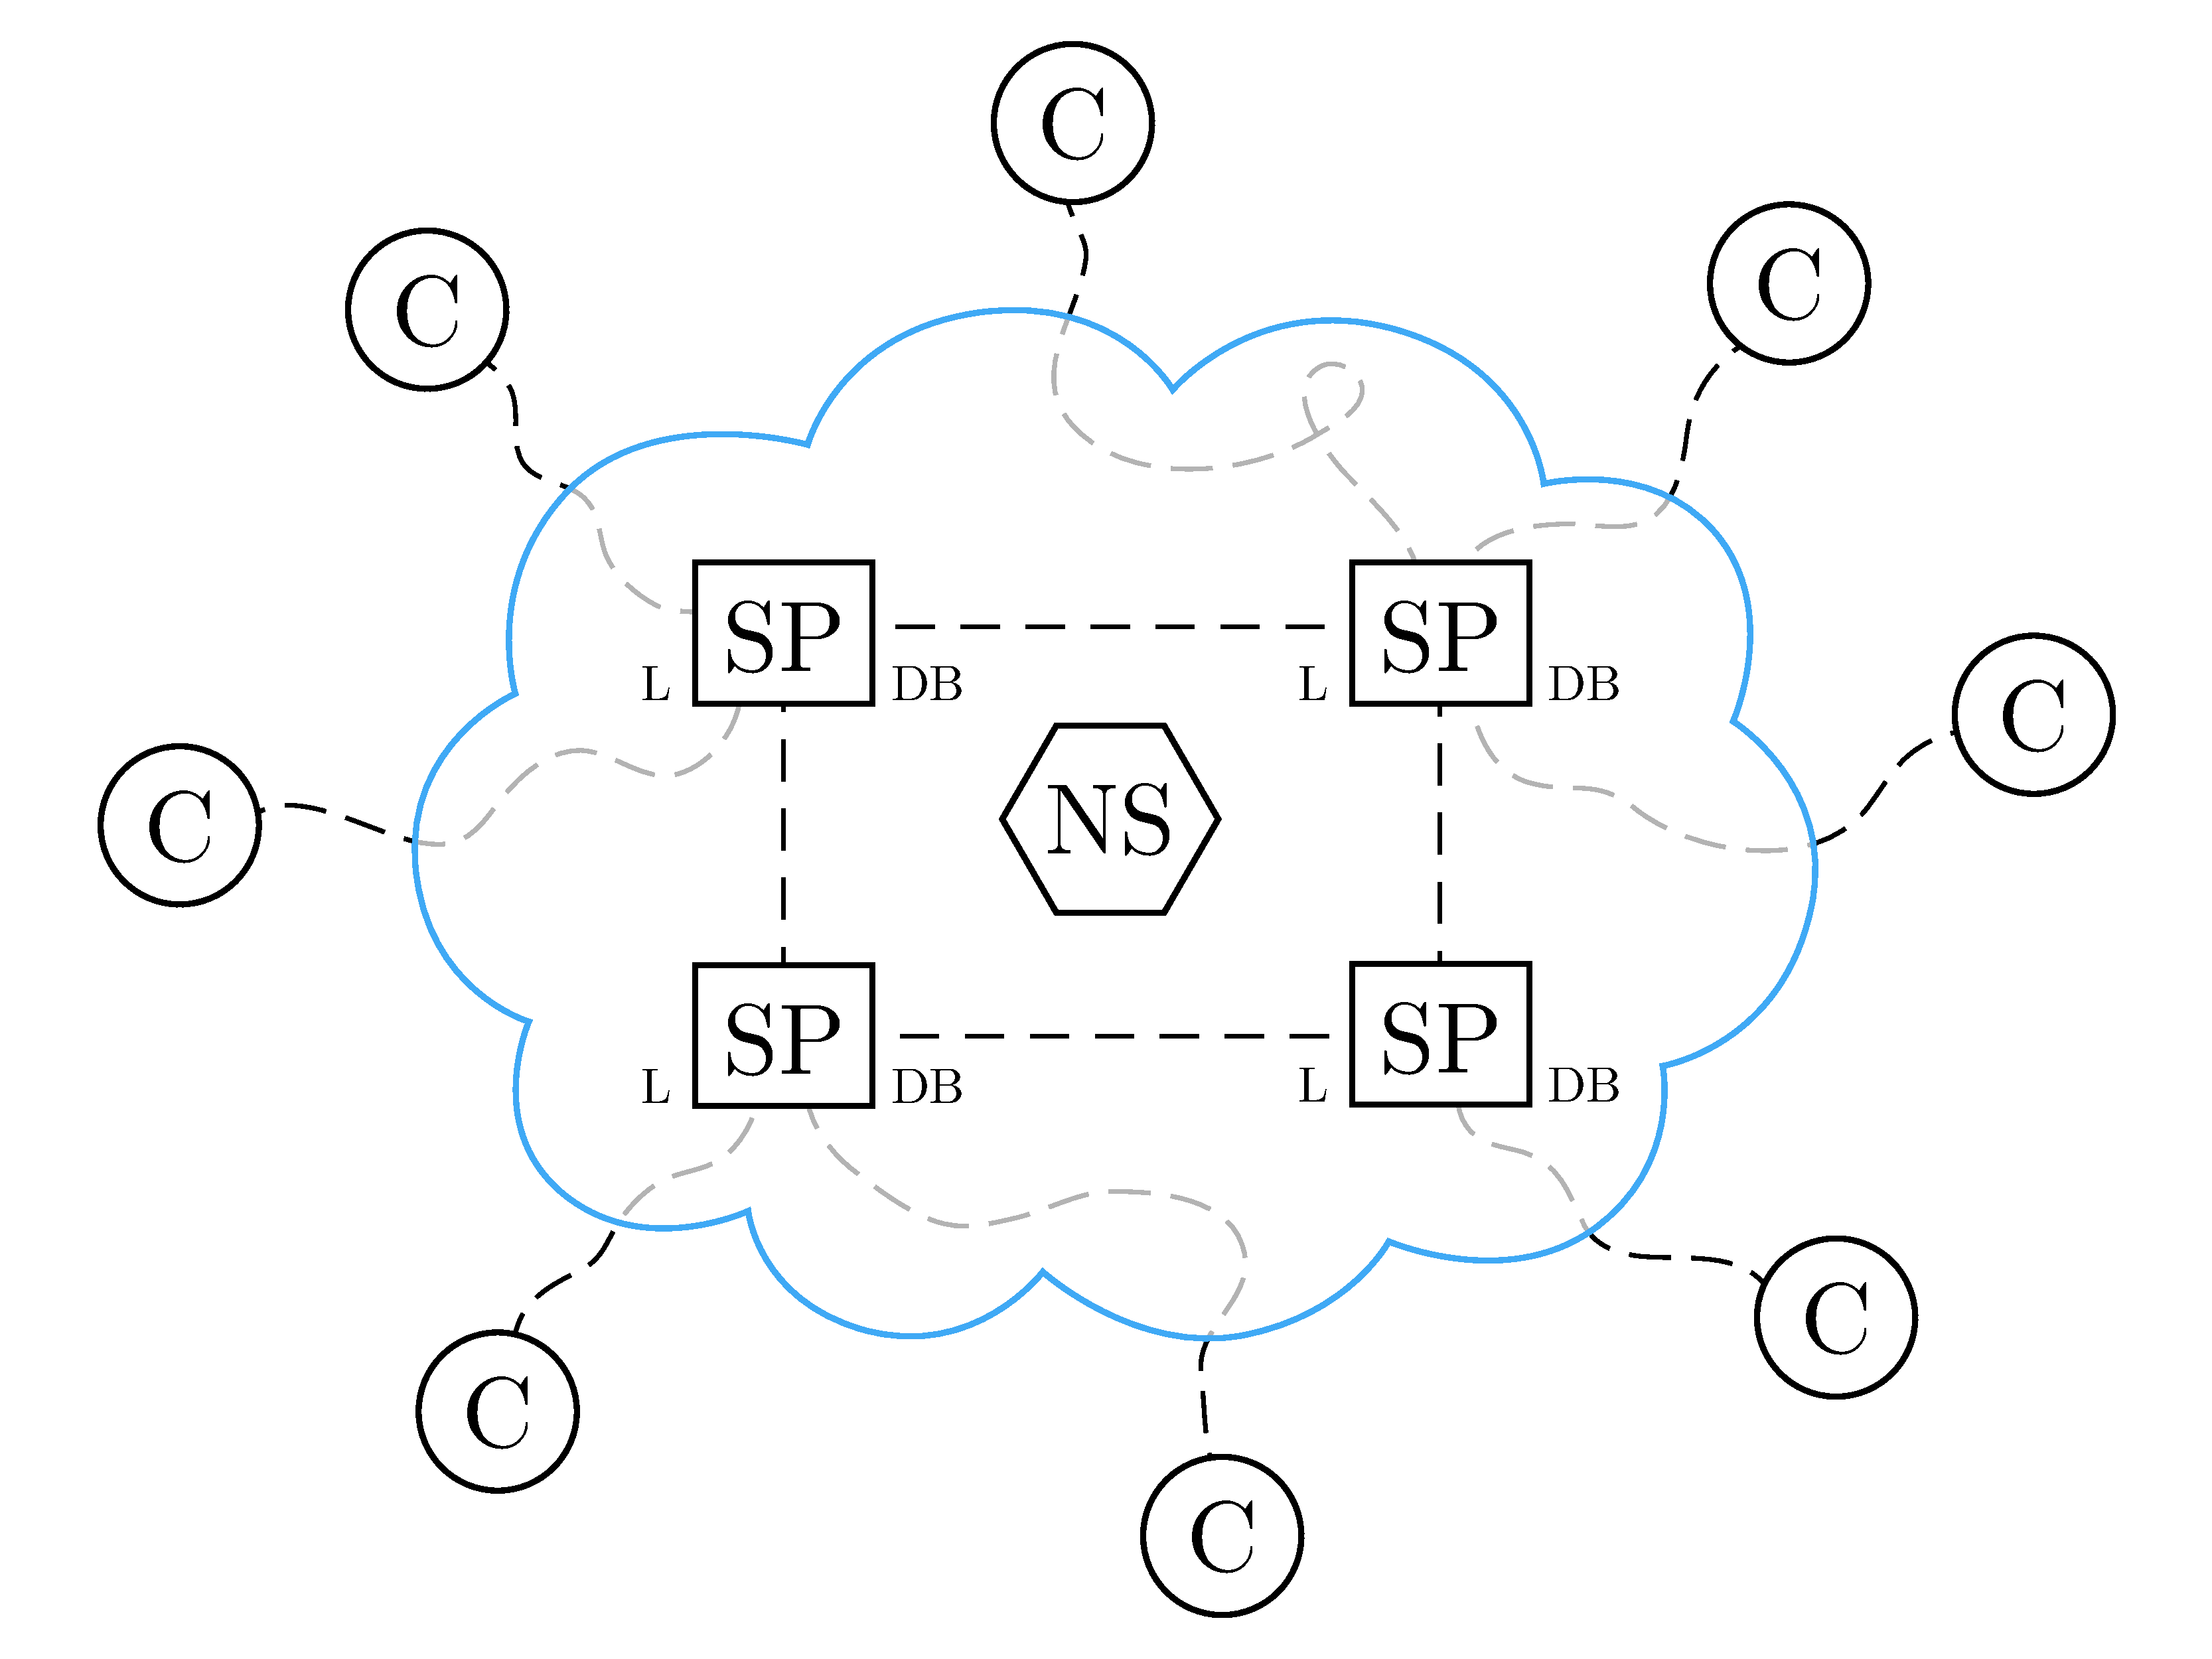
\includegraphics[scale=0.14,page=1]{include/assets/distributed-database}
  \column{3cm}
  \begin{tabular}{l @{ --- } l}
    \alert{C}  & client \\
    \alert{SP} & server/peer \\
    \alert{NS} & name service \\
    \alert{DB} & database \\
    \alert{L}  & lock
  \end{tabular}
\end{columns}
\end{frame}

\begin{frame}{Lab 0: Standalone Database}
  \centering
  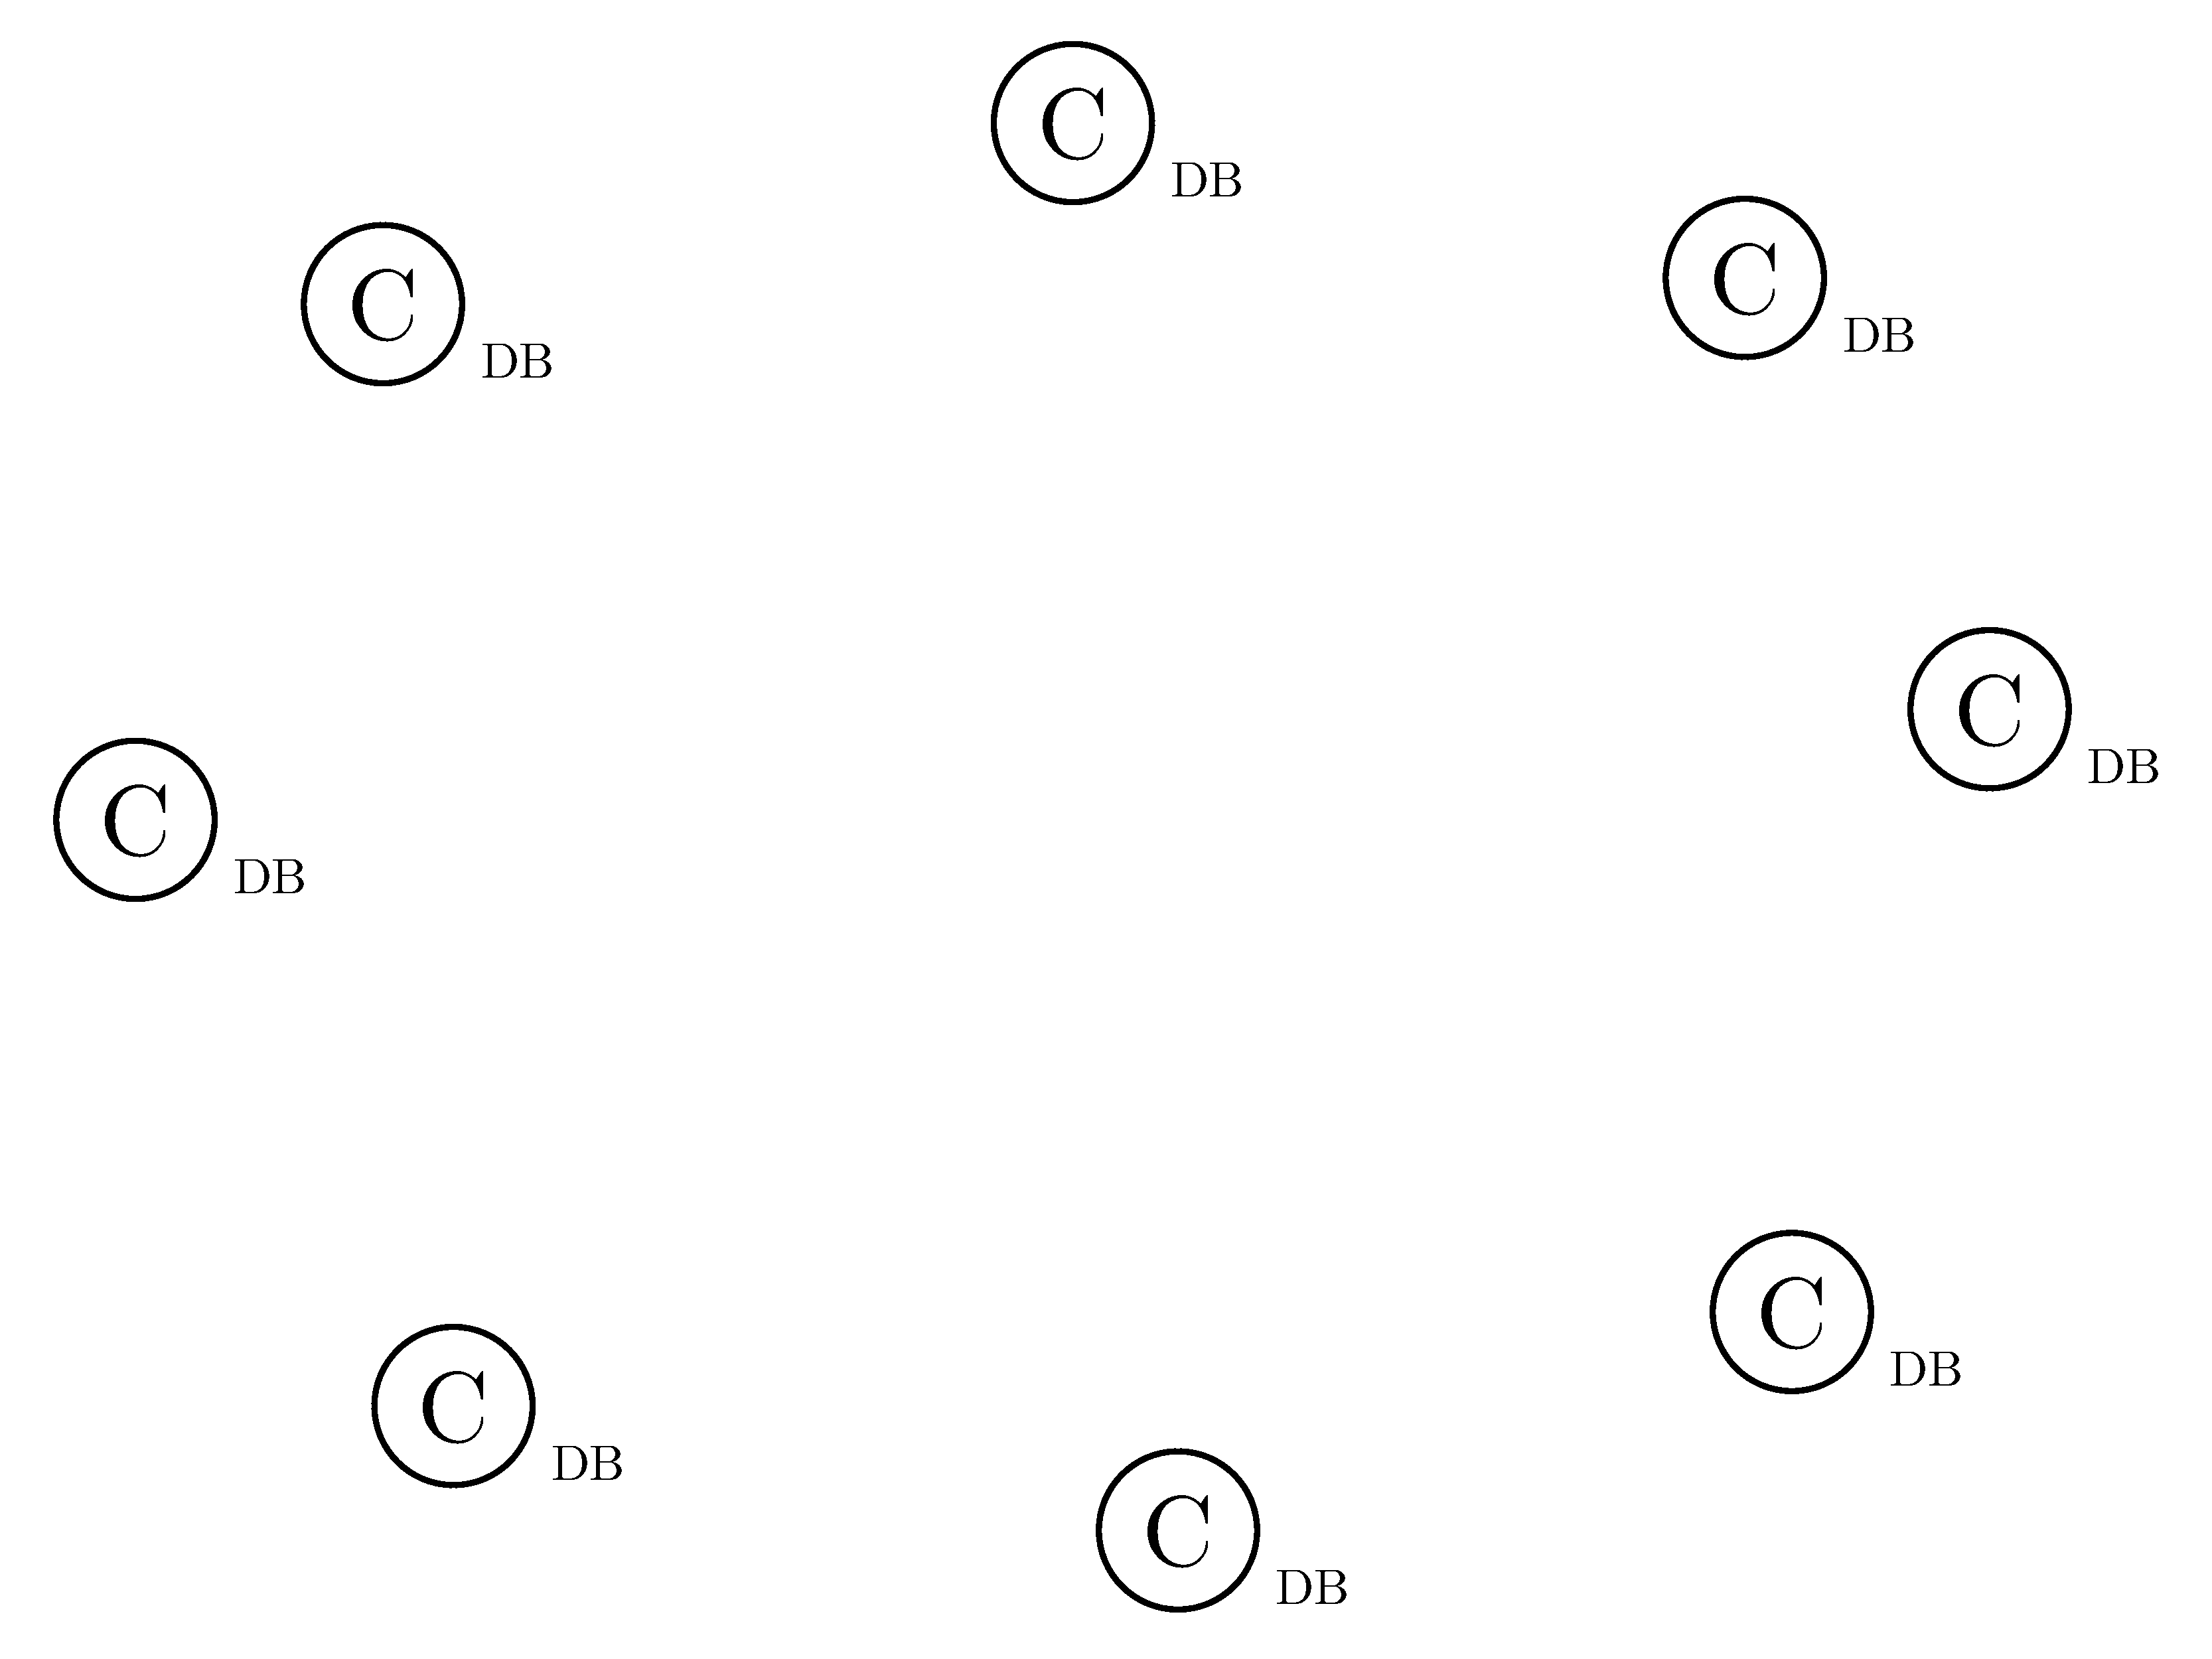
\includegraphics[scale=0.10,page=1]{include/assets/standalone-agents}
  \vspace{0.5em}
  \begin{itemize}
    \item Local database for each client
    \item \alert{TODO}: complete the implementation of the read and write
    operations of the database
  \end{itemize}
  \begin{center}
    \scriptsize \url{https://gitlab.ida.liu.se/tddd25/labs/raw/master/doc/lab0.pdf}
  \end{center}
\end{frame}

\begin{frame}{Lab 1: Client-Server Database}
  \centering
  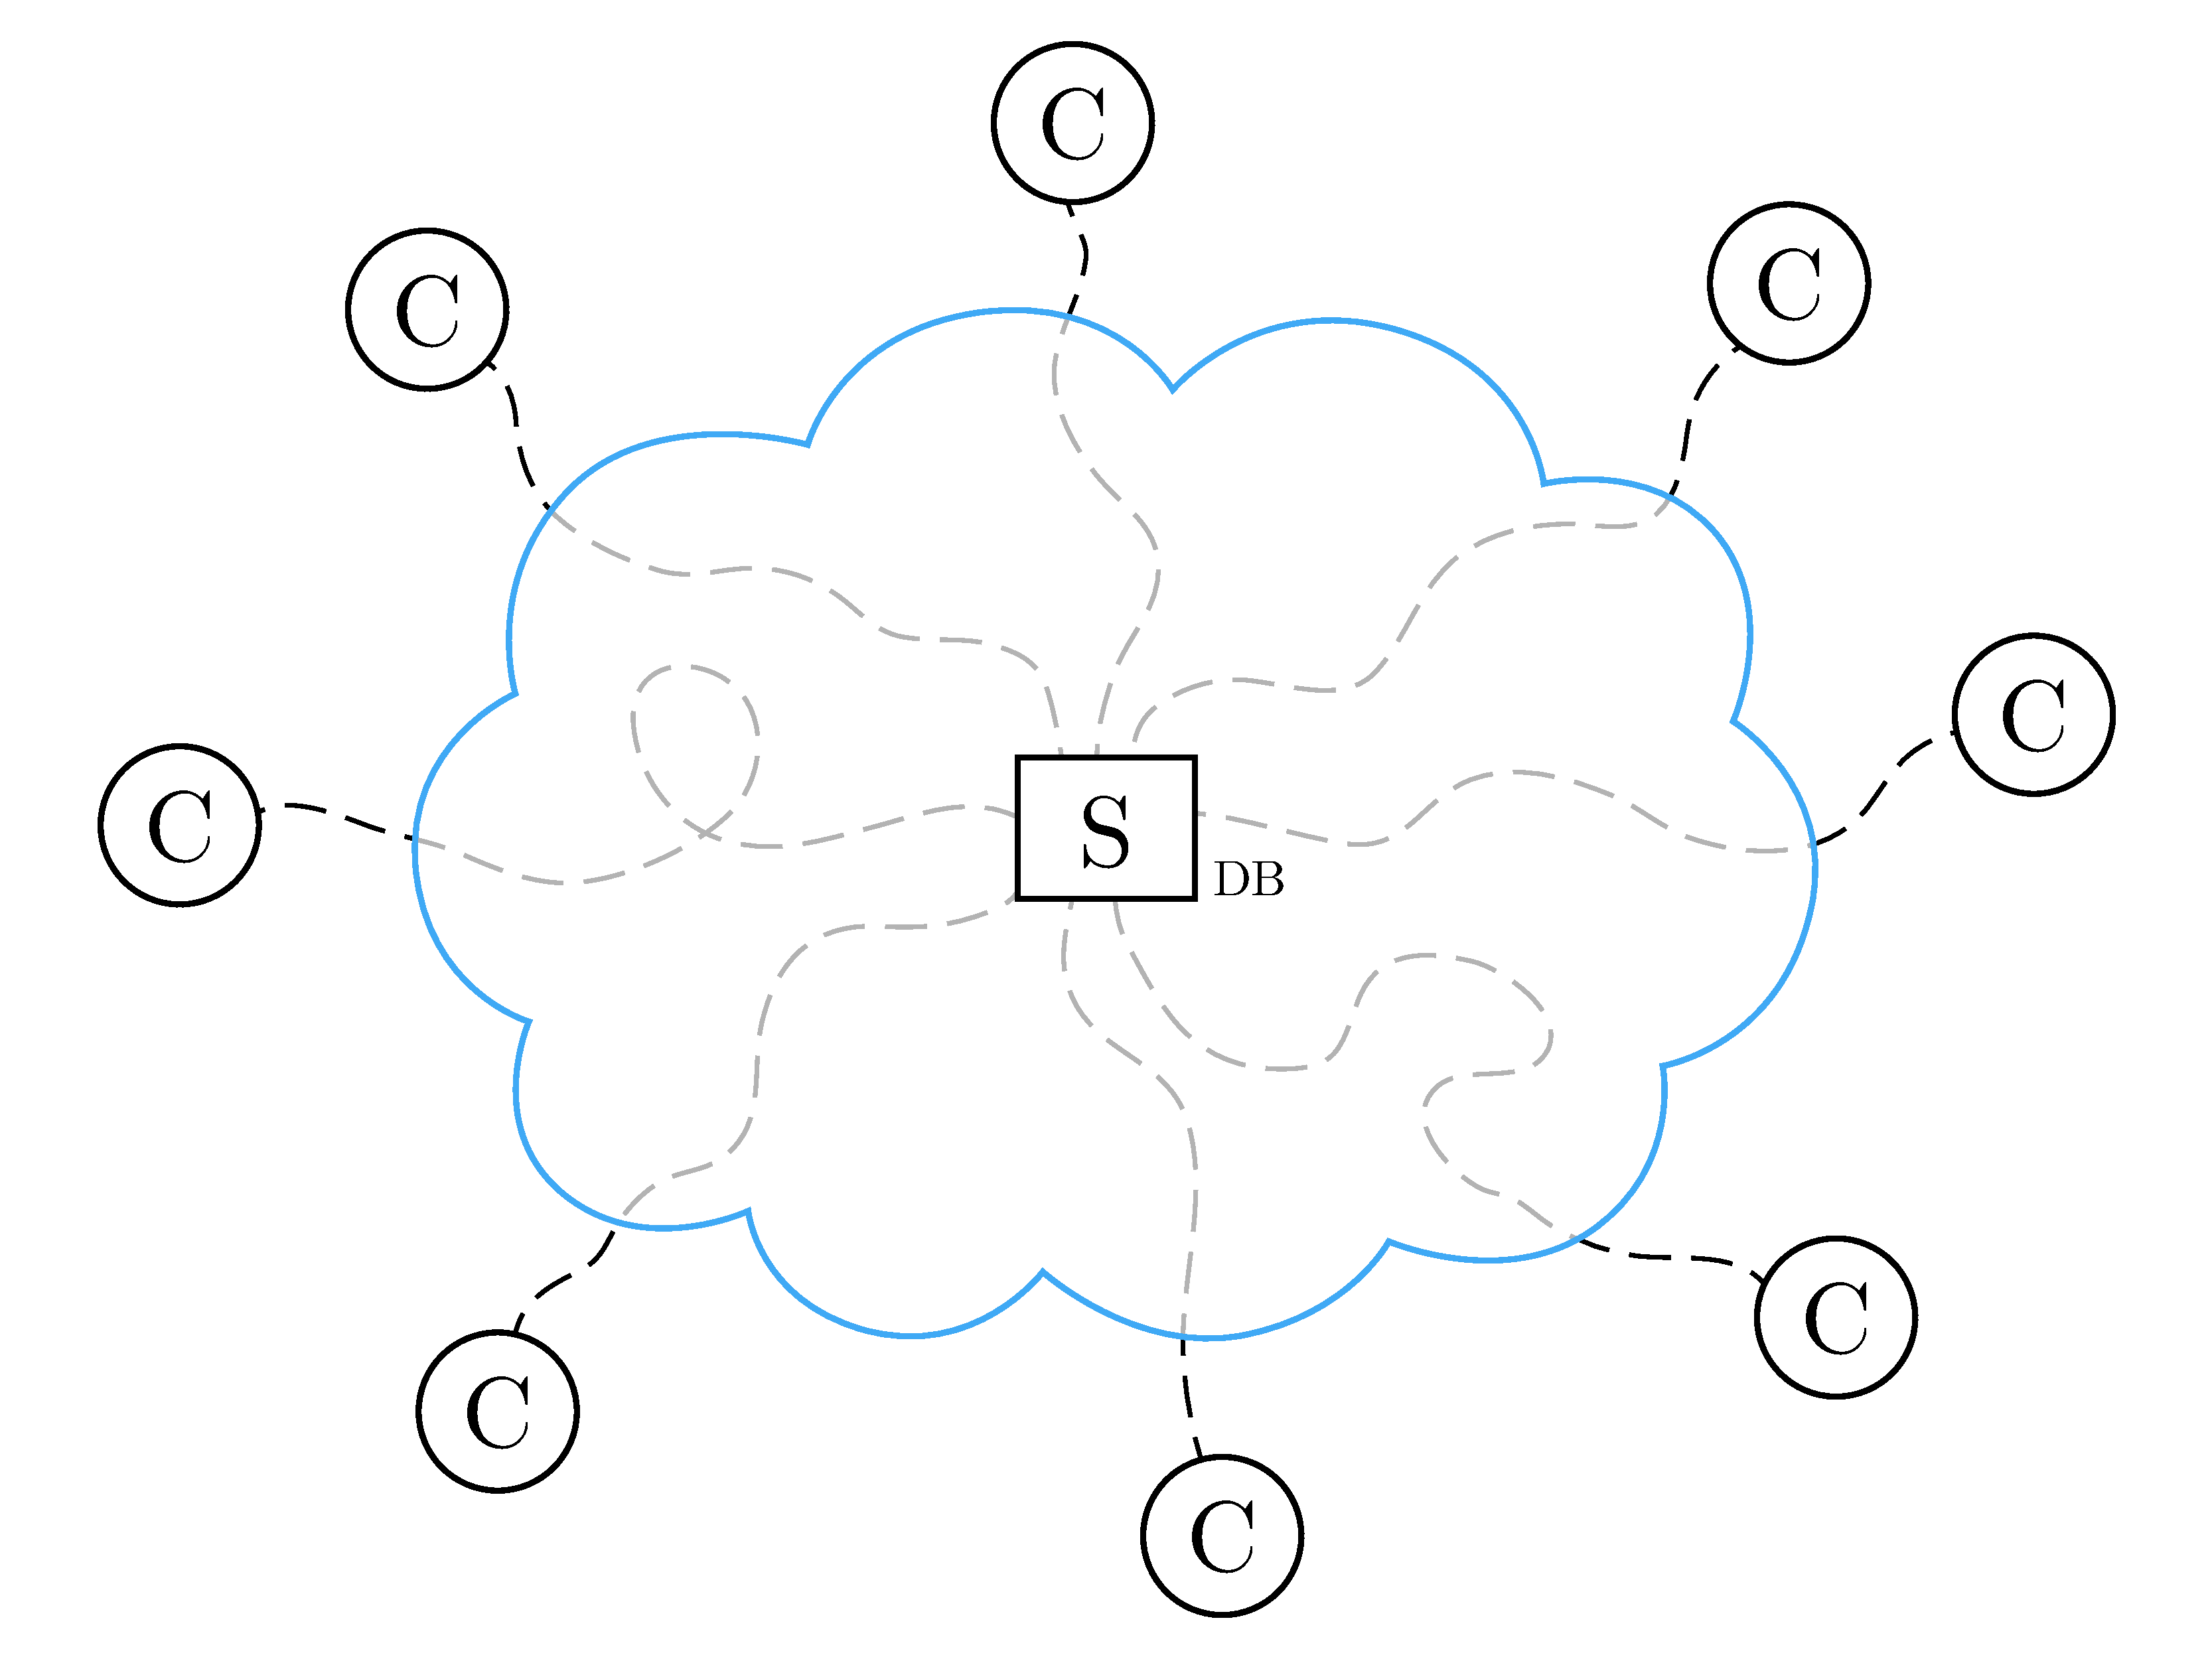
\includegraphics[scale=0.10,page=1]{include/assets/single-server}
  \begin{itemize}
    \item Centralized database
    \item \alert{TODO}: complete the implementation of the client/server
    communication mechanism
  \end{itemize}
  \begin{center}
    \scriptsize \url{https://gitlab.ida.liu.se/tddd25/labs/raw/master/doc/lab1.pdf}
  \end{center}
\end{frame}

\begin{frame}{Lab 2: Object Request Broker}
  \centering
  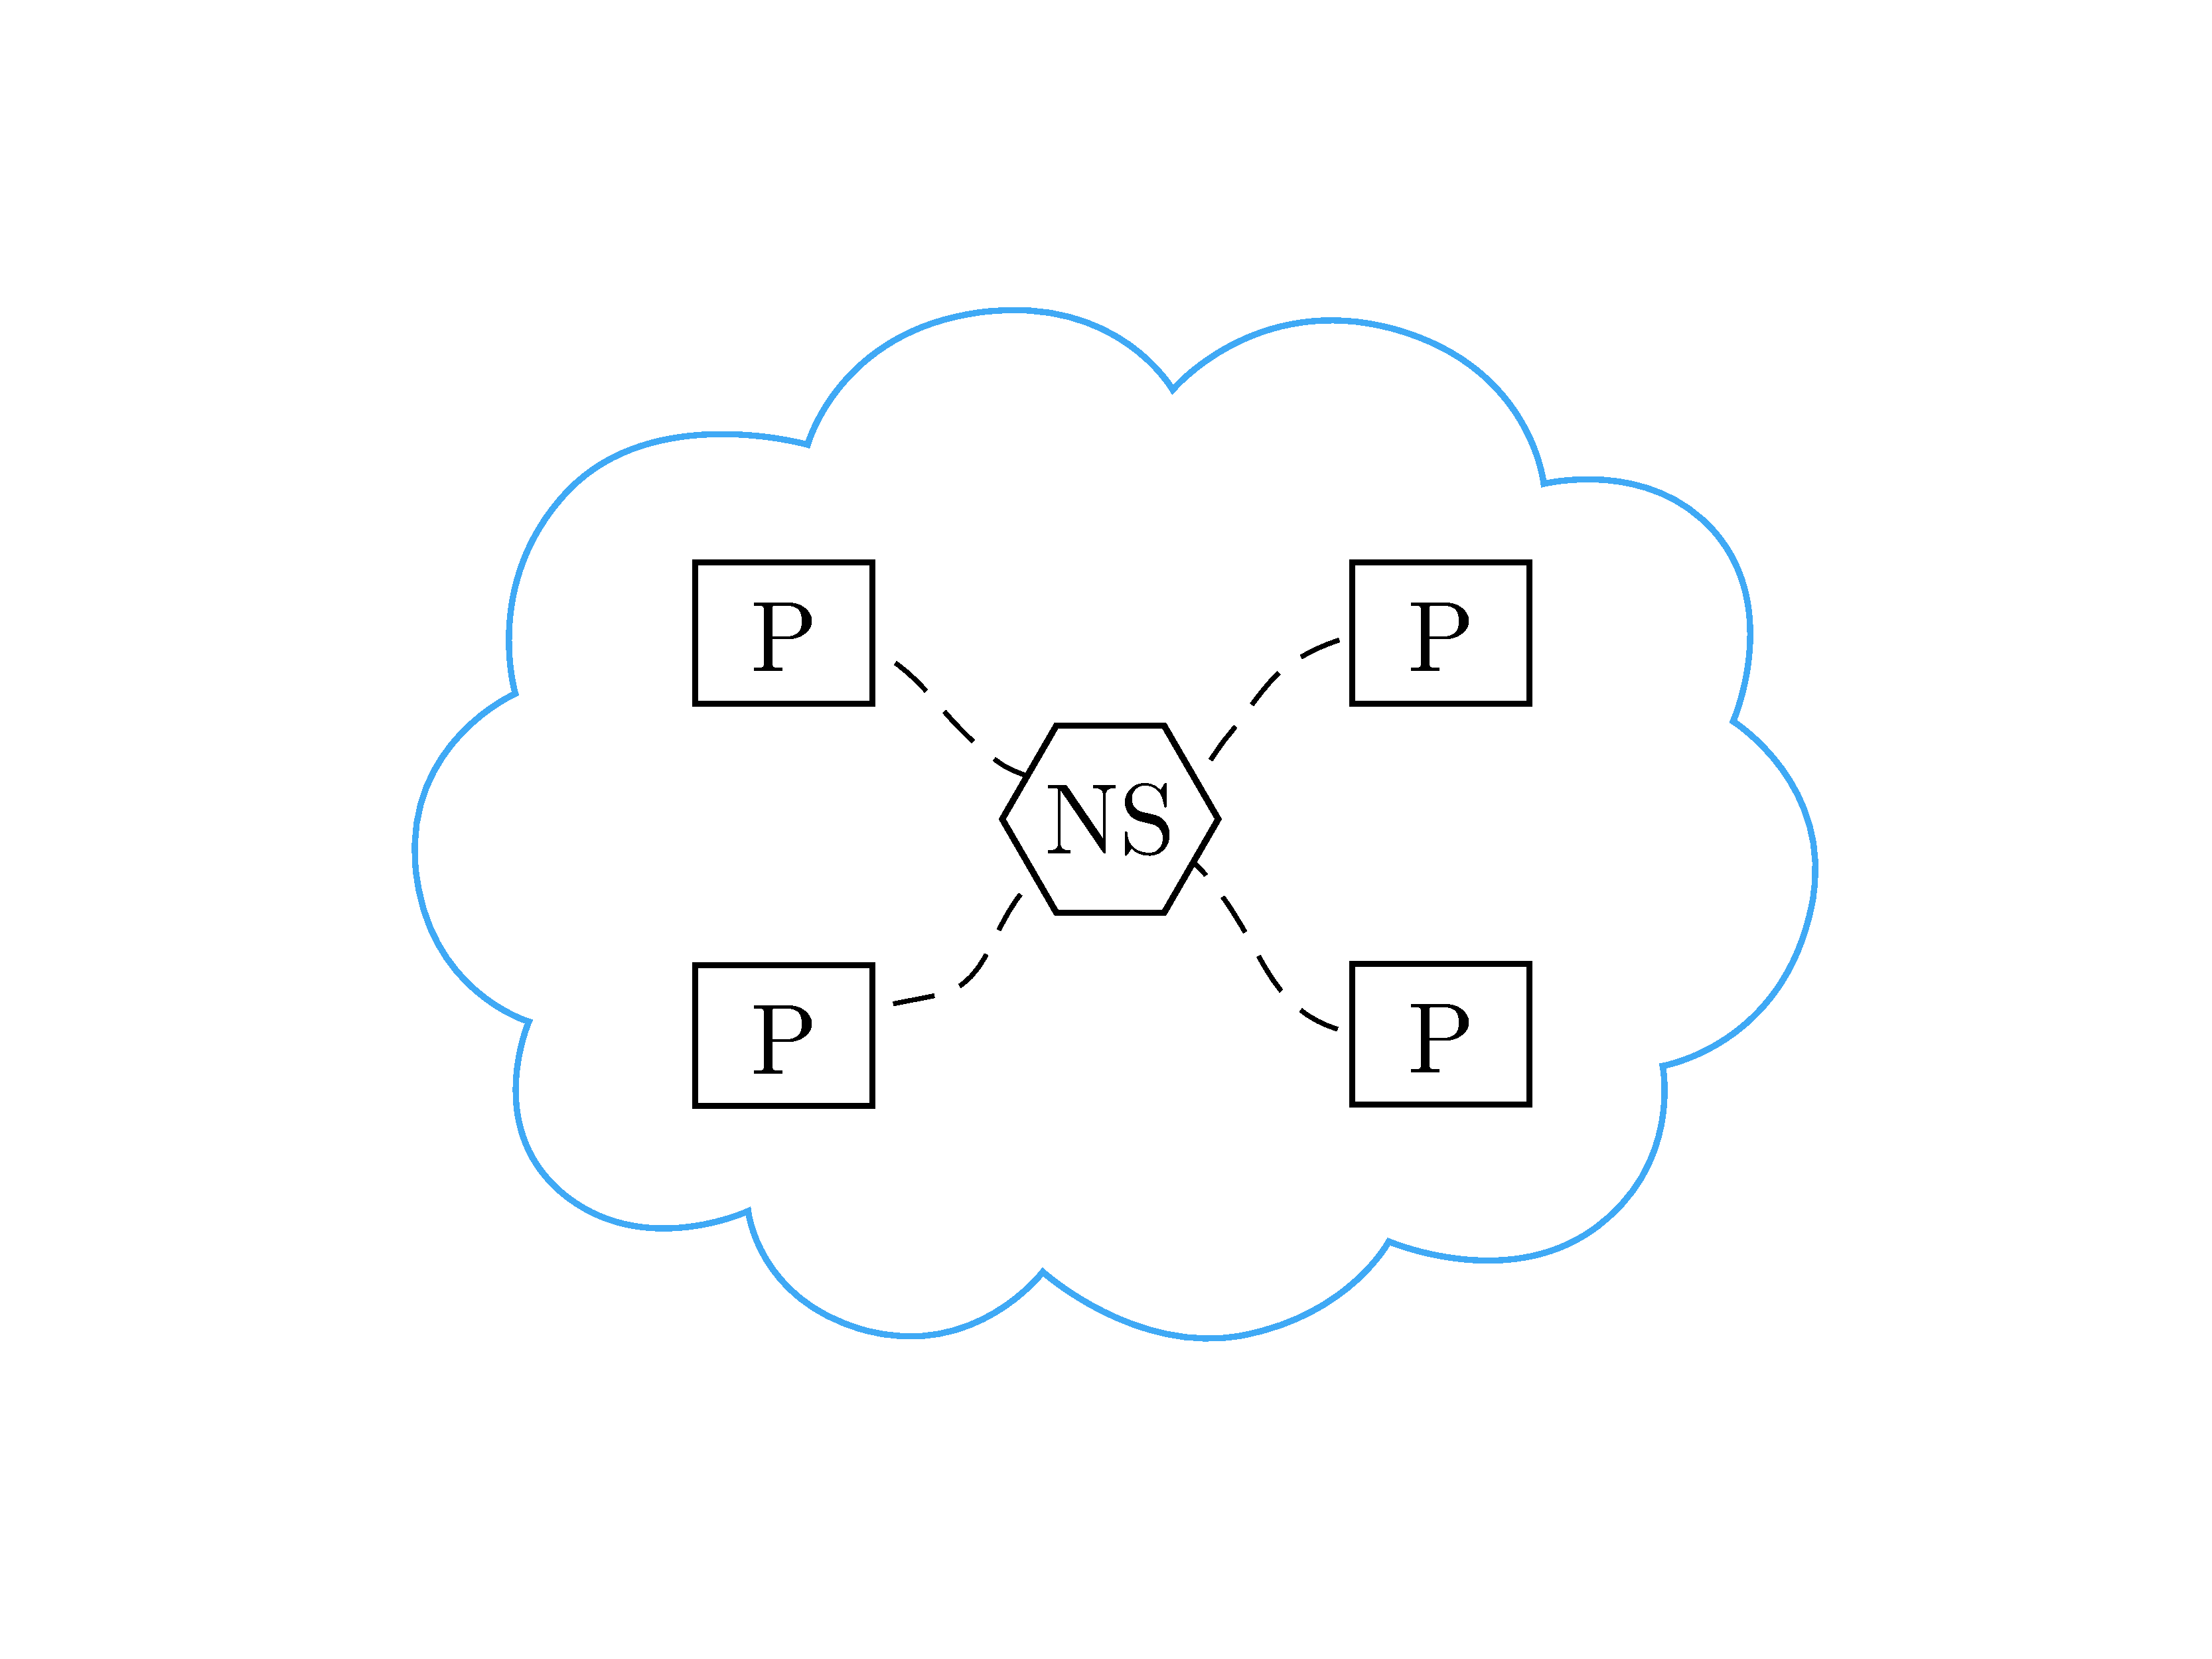
\includegraphics[scale=0.10,page=1]{include/assets/name-service}
  \begin{itemize}
    \item Name service and object request broker (ORB)
    \item Abstract away the communication part of the functionality
    \item \alert{TODO}: complete the implementation of the ORB
  \end{itemize}
  \begin{center}
    \scriptsize \url{https://gitlab.ida.liu.se/tddd25/labs/raw/master/doc/lab2.pdf}
  \end{center}
\end{frame}

\begin{frame}{Lab 3: Peer-to-Peer Communication}
  \centering
  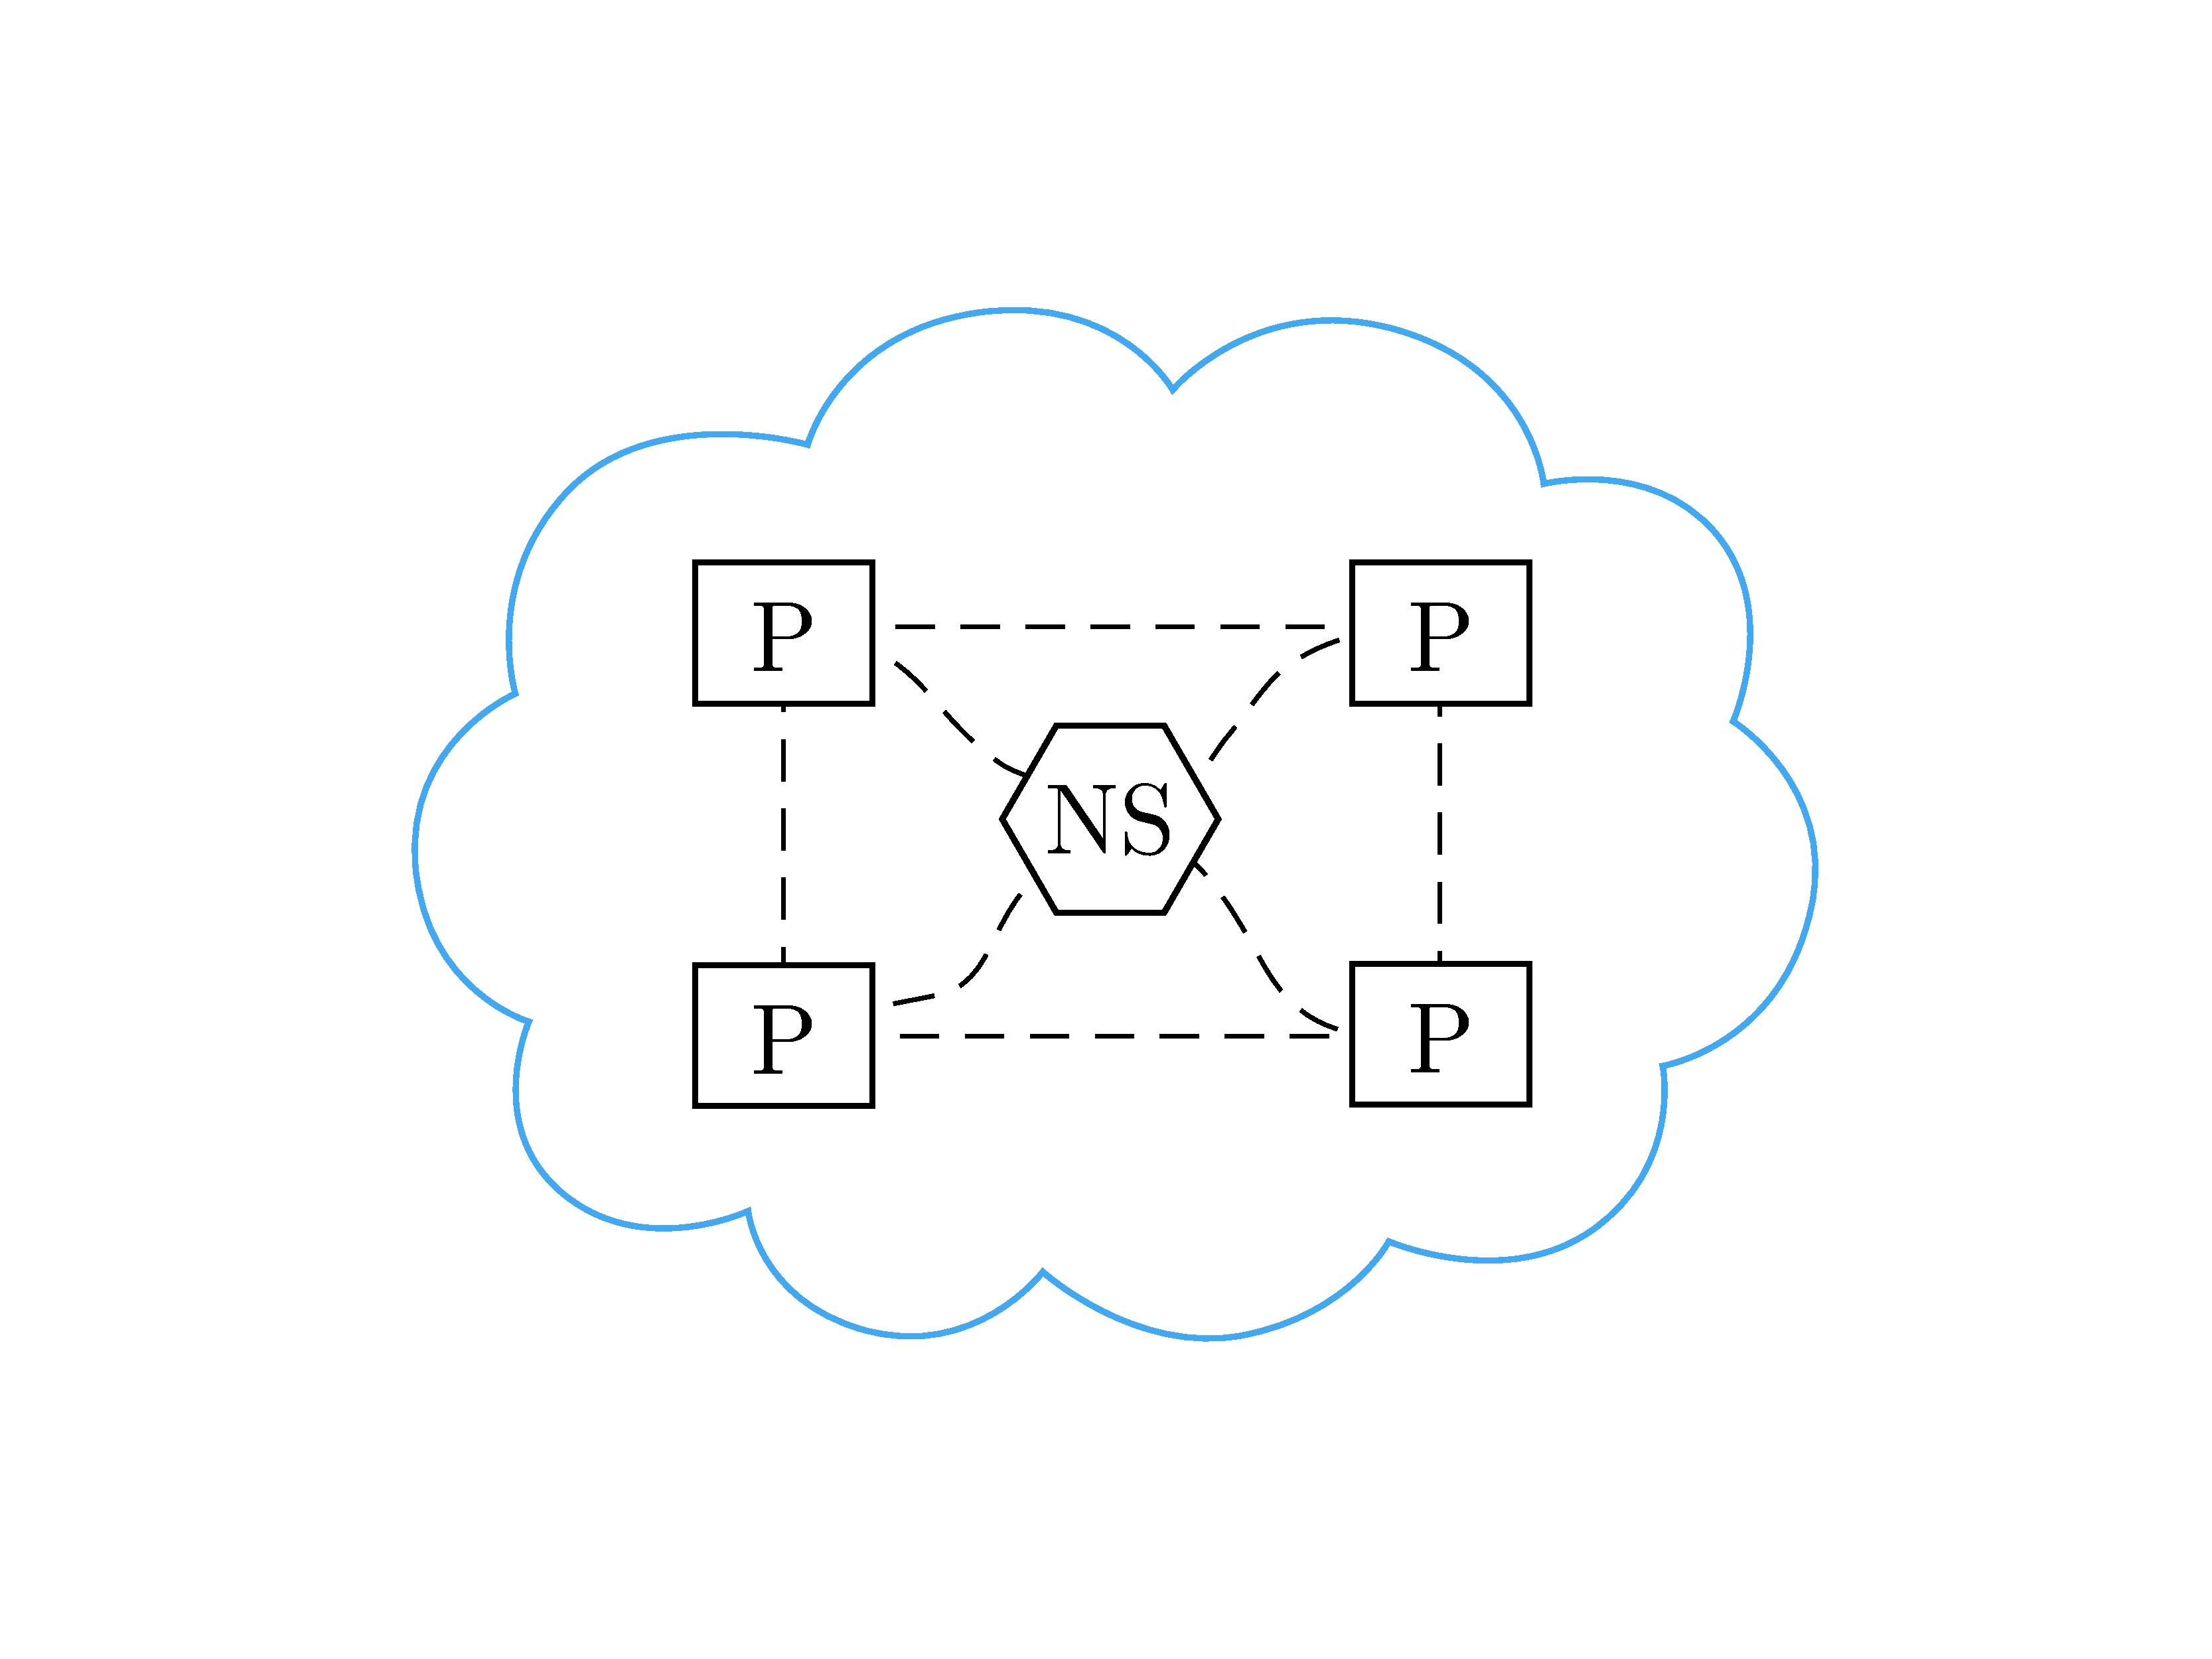
\includegraphics[scale=0.10,page=1]{include/assets/chat}
  \begin{itemize}
    \item Smart mechanism for keeping track of peers
    \item \alert{TODO}: complete the functionality dealing with the peers
    joining or leaving the system
  \end{itemize}
  \begin{center}
    \scriptsize \url{https://gitlab.ida.liu.se/tddd25/labs/raw/master/doc/lab3.pdf}
  \end{center}
\end{frame}

\begin{frame}{Lab 4: Distributed Locks}
  \centering
  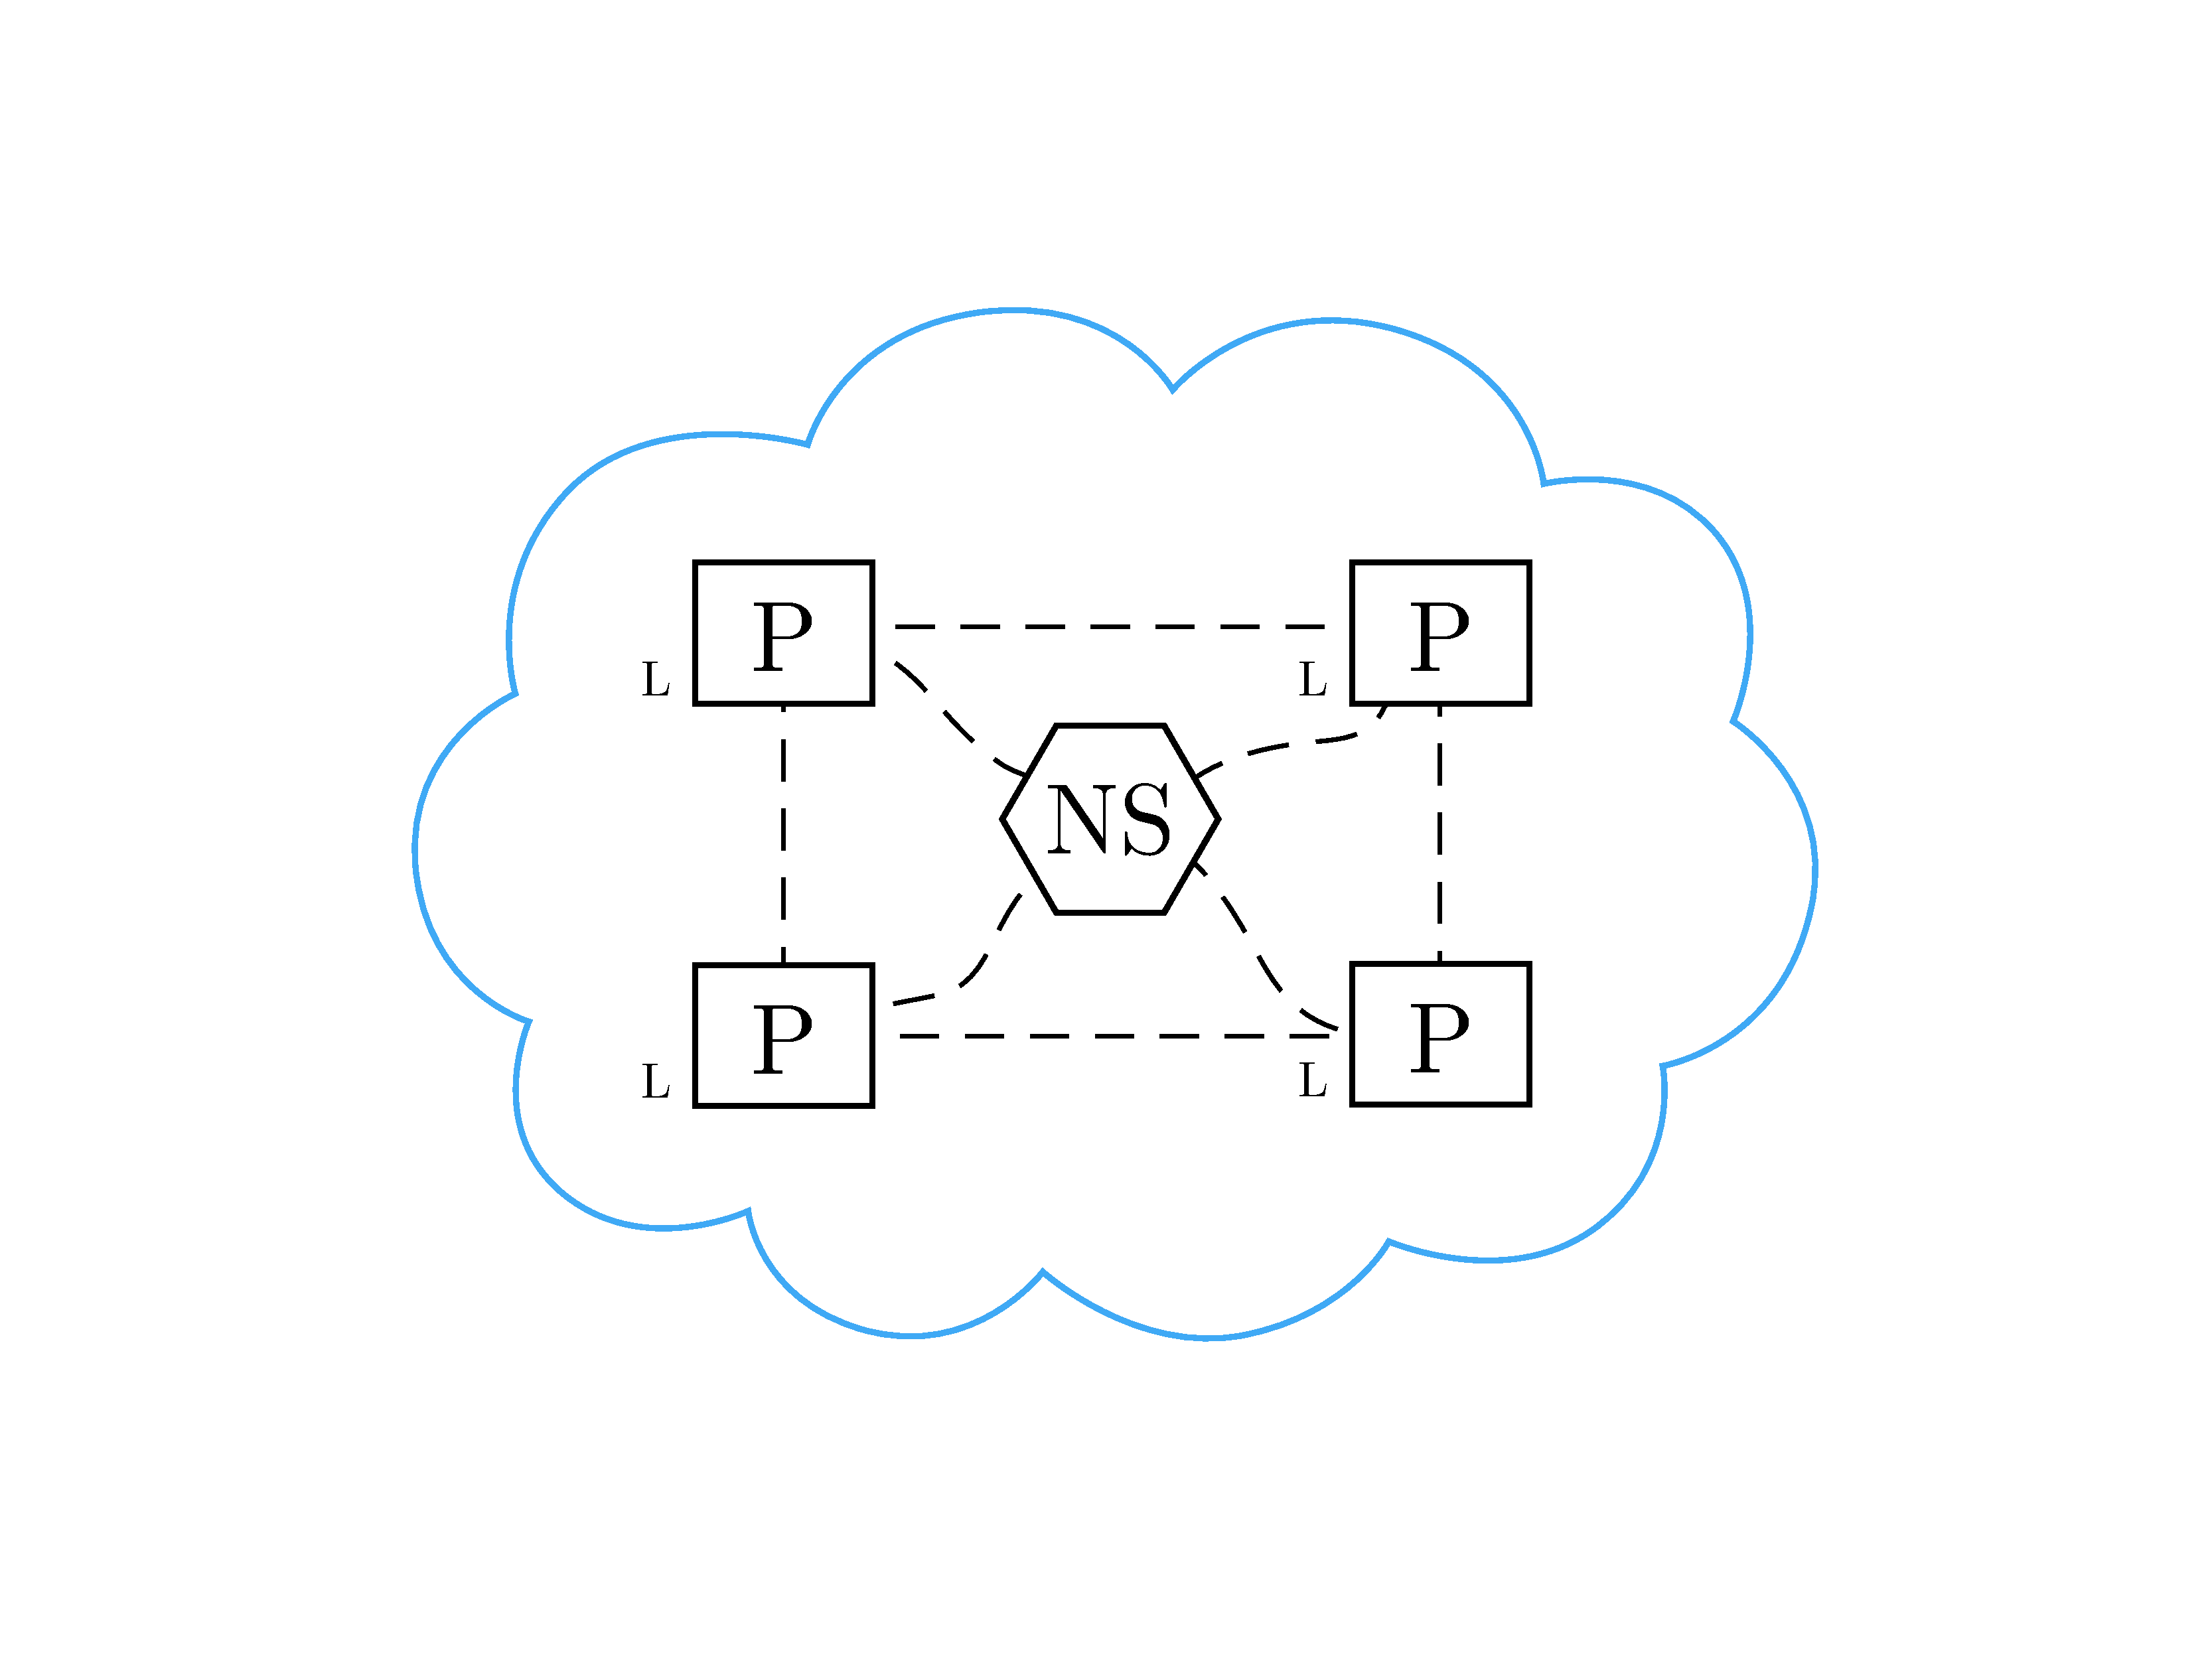
\includegraphics[scale=0.10,page=1]{include/assets/lock}
  \begin{itemize}
    \item Distributed mutual exclusion to control concurrent operations
    \item \alert{TODO}: complete the implementation of the second
    Ricart--Agrawala algorithm
  \end{itemize}
  \begin{center}
    \scriptsize \url{https://gitlab.ida.liu.se/tddd25/labs/raw/master/doc/lab4.pdf}
  \end{center}
\end{frame}

\begin{frame}{Lab 5: Client-Server Database with Replicas}
  \centering
  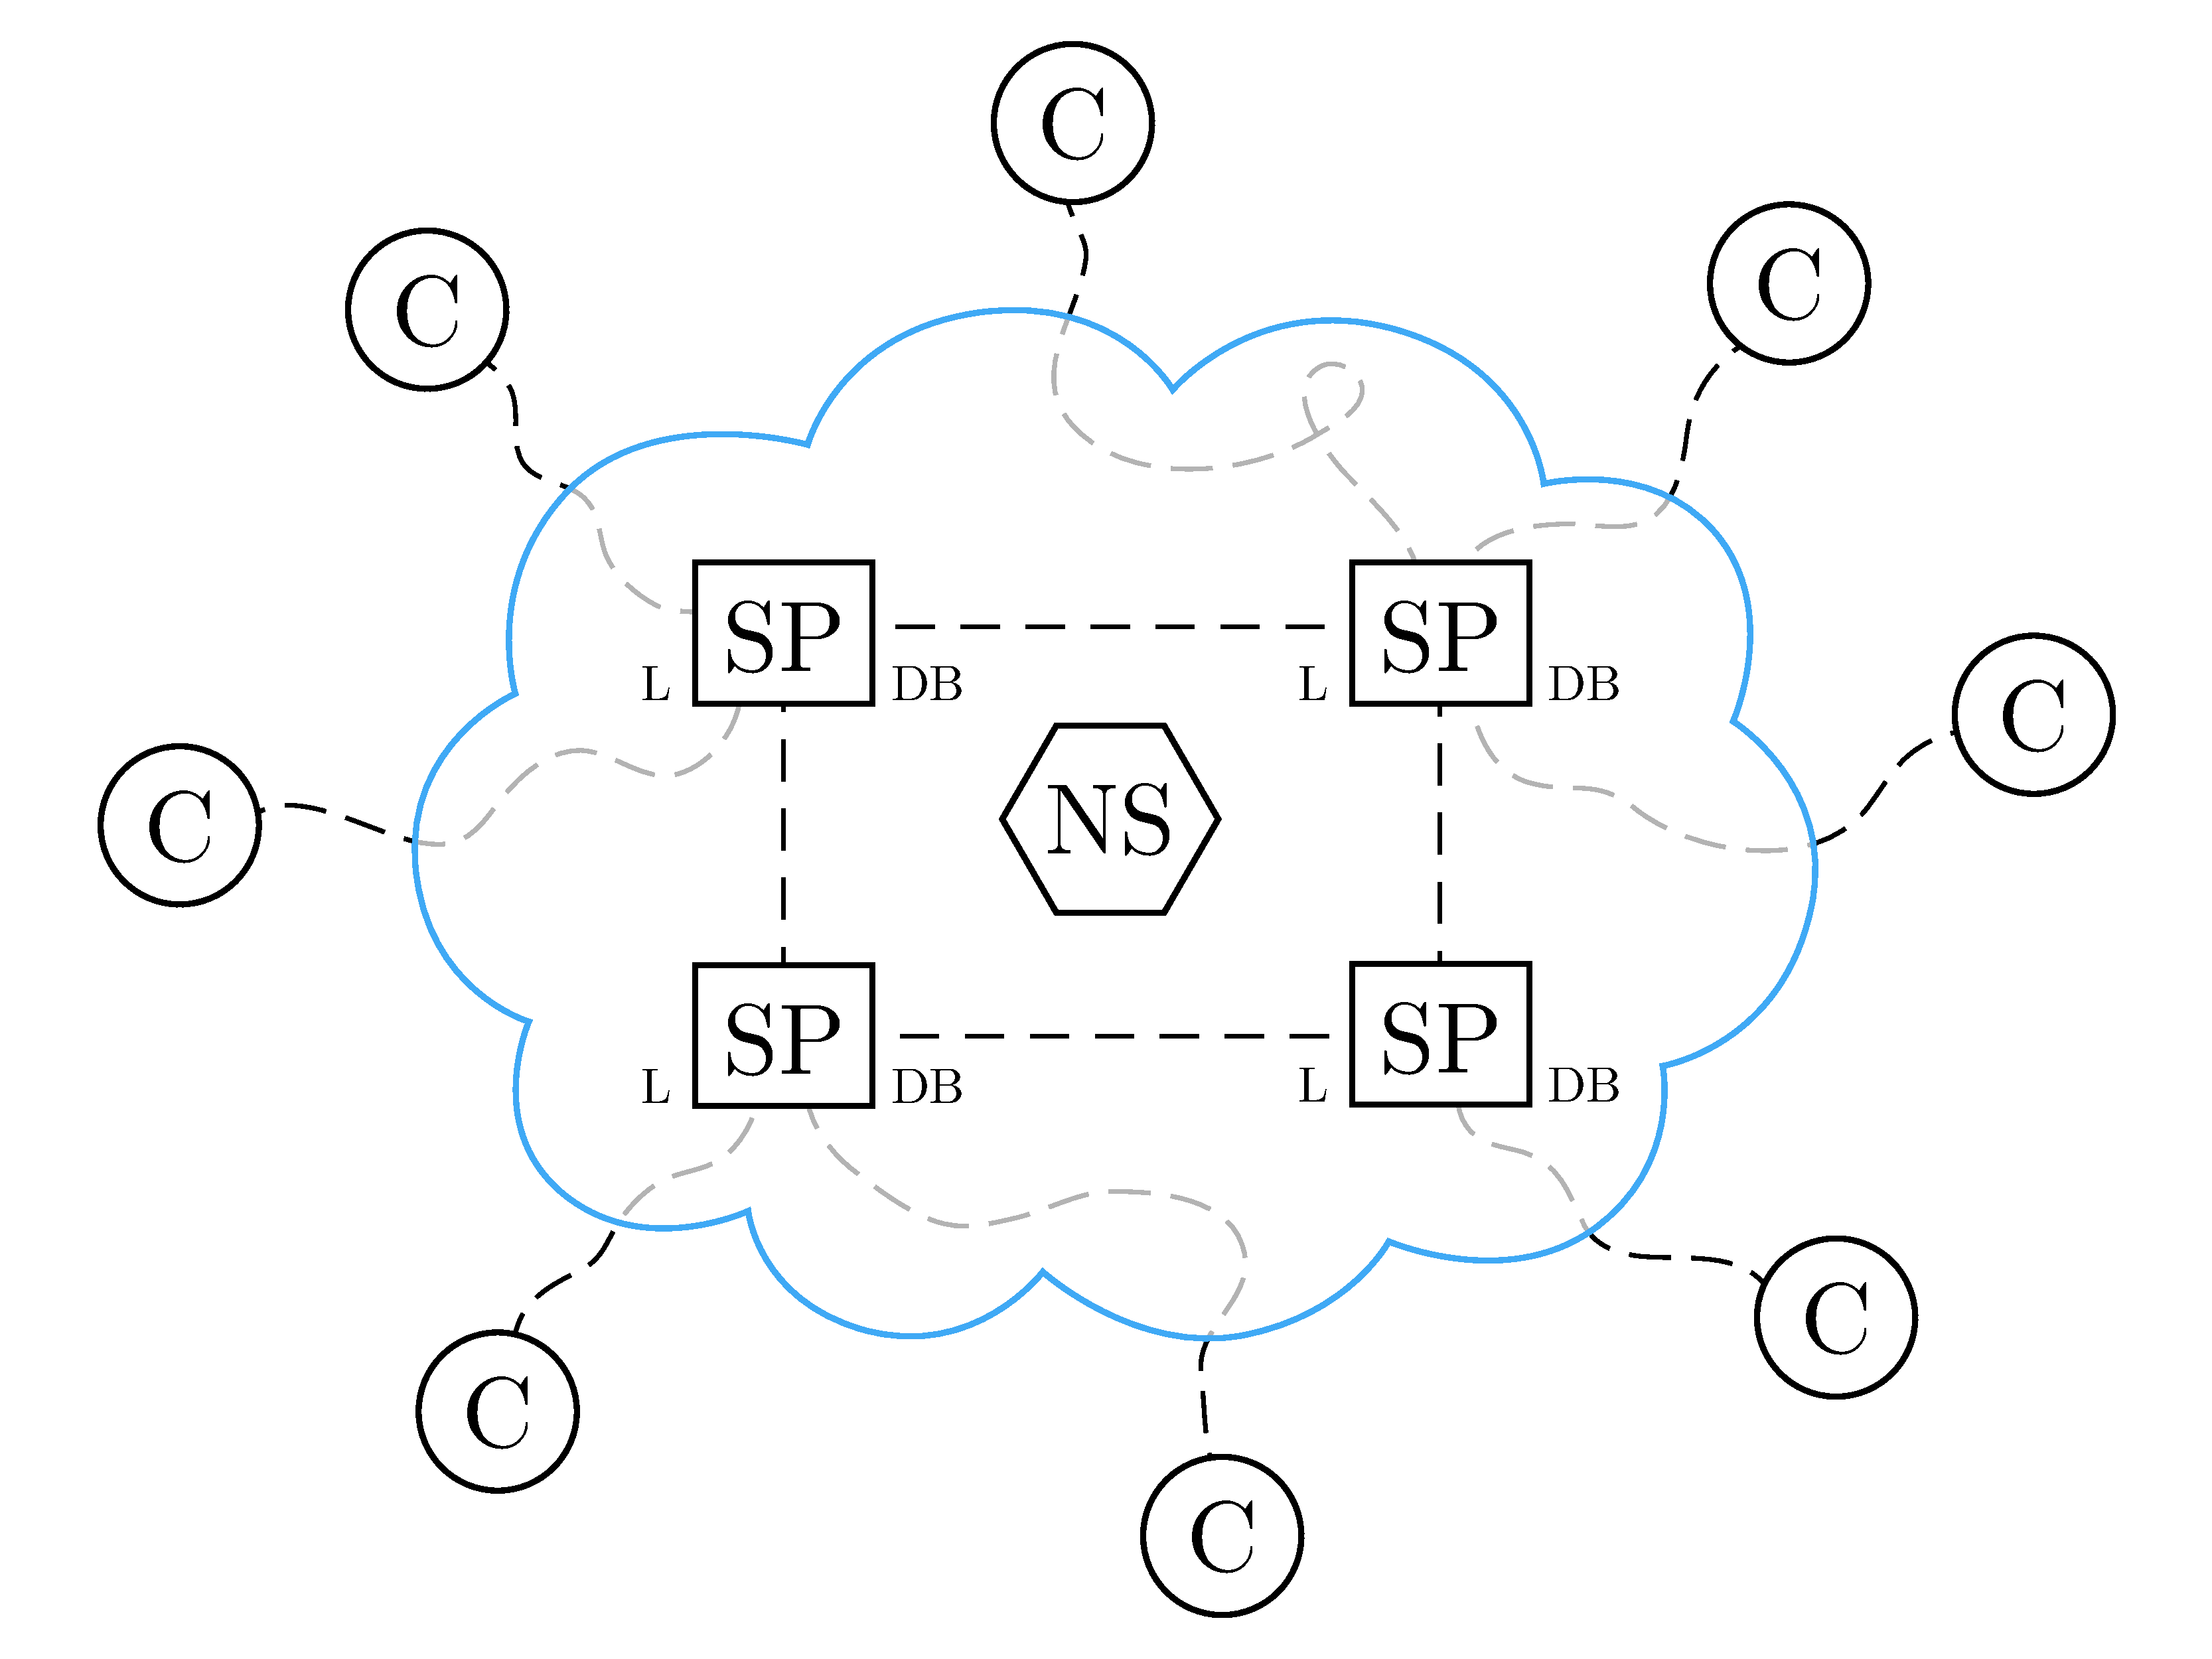
\includegraphics[scale=0.10,page=1]{include/assets/distributed-database}
  \begin{itemize}
    \item Everything together
    \item \alert{TODO}: complete the implementation of the server/peer using all the previously developed components
  \end{itemize}
  \begin{center}
    \scriptsize \url{https://gitlab.ida.liu.se/tddd25/labs/raw/master/doc/lab5.pdf}
  \end{center}
\end{frame}

\begin{frame}{Implementation}
  \begin{itemize}
    \item Multi-threaded object-oriented code in Python 3
    \item Communication via objects serialized in JSON
    \item Data transfer through TCP sockets
  \end{itemize}
\end{frame}

\begin{frame}{Repository}
  \centering
  \begin{itemize}
    \item doc/
    \item src/
      \begin{itemize}
        \item lab0/
        \item lab1/
        \item lab2/
        \item lab3/
        \item lab4/
        \item lab5/
        \item modules/
          \begin{itemize}
            \item Common/
            \item Server/
          \end{itemize}
      \end{itemize}
  \end{itemize}
\end{frame}

\begin{frame}{Submission}
  \centering
  \begin{itemize}
    \item No written reports are needed
    \item Demonstrate your solutions in class
    \item Email modified files
  \end{itemize}
\end{frame}

\begin{frame}
  \vspace{3em}
  \begin{center}
    {\huge Good luck!}
  \end{center}
\end{frame}

\end{document}
